\section{Det diskrete logaritmeproblem}
I følgende afsnit redegøres der for det diskrete logaritmeproblem, hvorefter en algoritme til at løse problemet opstilles. Efter dette sammenlignes tidsforbruget af algoritmen med tiden for at generere en offentlig nøgle. 

Hvis MITM vil bryde krypteringen, går det ud på at løse det nedenstående problem.
\begin{mdframed}[frametitle={Det diskrete logaritmeproblem for elliptiske kurver}]
Givet to punkter $A$ og $G$ find heltallet $\alpha$ som opfylder ligningen:
\begin{equation}
    A=\alpha \cdot G
\end{equation}
Hvor $\alpha$ er et helt tal og $G$ og $A$ er gruppeelementer.
\end{mdframed}

Dette problem kaldes for: Det diskrete logaritmeproblem for ECC og siges at være et \textit{”svært problem”}, da der ikke findes nogen algoritme som kan løse det på en bestemt polynomisk tid, som kan køre på en \textit{”normal”} computer (\cite{youssefelhousni2018}). Det er dog vigtigt at sige, at der ikke til dags dato, findes et bevis for at forrige postulat er sandt (\cite{timsroberts}). Umiddelbart har navnet: Det diskrete logaritmeproblem ingen sammenhæng med elliptiske kurver, men det skyles at det stammer fra andre grupper hvor man i stedet bruger \textit{multiplikativ} notation hvor ligningen opskrives som $A=G^\alpha  \pmod{p}$. Her skriver vi løsningen  som $log_{G}A=\alpha$. Vi kigger nu på gruppen for $Z_p \backslash {0}$ hvor $p$ er et stort primtal. Vi ved at den har $p-1$ elementer. At lave en algoritme til at løse dette problem er ikke særligt svært, da vi skal udregne $2G, 3G, 4G$ indtil at et af dem bliver lig med $A$.
\\\\
\begin{python}
	def brute_force(G, public_key, p):
		temp_point = G
		for i in range(1, p):
			if temp_point == public_key:
				return(i)
			temp_point = mult(i+1, G)
\end{python}
Overstående algoritme går iterativt igennem alle heltal fra 1 til $p$ indtil at $iG$ er lig med den offentlige nøgle.
Algoritmen vil stoppe efter $log_{G}A$ iterationer, og vi kan hermed løse problemet forholdsvist nemt til tiden $O(n)$, hvor $n$ er ordenen af $G$. Da en computer kan udføre ekstremt mange operationer meget hurtigt, kan vi kun bruge grupper med rigtigt store ordener. Vi kan fx, kigge på hvis $n > 2^{100}$, svarende til et tal som er 100 bit langt. Vi antager nu at en computer kan lave 1 milliard operationer svarende til ca. $2^{30}$ operationer pr sekund. Vi får at det vil tage $3,75\cdot 10^{13}\cdot$ år altså over 1 billion år at udregne $2^{100}$. Denne \textit{”brute-force”} algoritme kan altså ikke anvendes i praktisk når $n > 2^{100}$.


Hvad så med den anden vej når vi skal udregne $\alpha \cdot G$? Dette er ikke svært grundet vores double-and-add algoritme som tidligere beskrevet, hvor vi reducerer tiden til $O(log_{2}n)$ i stedet for $O(n)$. I praksis vil det sige at hvis Alice og Bob vælger at lave deres private key en bit længere, skal de kun udføre to ekstra regneoperationer hver \textit{(double-and-add)}, mens MITM som prøver at bryde krypteringen skal bruge dobbelt så meget regnekraft pr. ekstra bit.


Det kan hermed ses at krypteringen vokser lineært i forhold til bitlængden $k$, hvor arbejdet ved at løse det diskrete logaritmeproblem i gruppen stiger eksponentielt med bitlængden. Til at vise følgende også gælder for virkeligheden, har jeg implementeret brute-force metoden i mit program. Ved at iterere over forskellige privat-nøgler med en step-size på $2^i$ kan vi lave et plot med bitlængden af privatnøglen samt tiden det tog at udregne. Python-biblioteket \code{timeit} blev anvendt

\begin{figure}[htbp]
\centering
\begin{subfigure}{.5\textwidth}
  \centering
  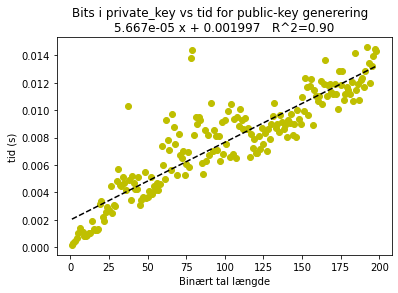
\includegraphics[width=1.0\linewidth]{images/gen.png}
  \caption{Public-Key generering (Double-and-Add)}
  \label{fig:sub1}
\end{subfigure}%
\begin{subfigure}{.5\textwidth}
  \centering
  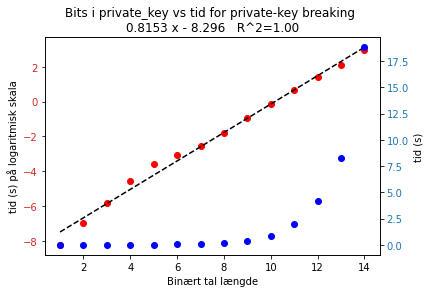
\includegraphics[width=1.0\linewidth]{images/breaking.png}
  \caption{Private-Key breaking (Naiv algoritme)}
  \label{fig:sub2}
\end{subfigure}
\caption{Modellering af generering vs. breaking af nøgler se \ref{section:figur_6} for kode}
\label{fig:genvsbreak}
\end{figure}

På \fref{fig:genvsbreak}a ses et punktplot af længden af privatnøglens længde i binær udaf førsteaksen, og tiden det tog at udregne på andenaksen. Udover det er der foretaget en lineær regression, hvor vi får modellen: $t_{gen}=5,667\cdot 10^{-5}\cdot k + 1,997\cdot 10^{-4}$ hvor $k$ er længden af det binære tal. Da vi får en $R^2=0,90$ kan vi konkludere at vores model er valid. Det kan dog ses at der generelt kommer en større afvigelse fra modellen når længden af det binære tal stiger. Vi udregner nu tiden det ville tage for en 100-bit lang private-key.
$$t_{gen} (100)=5,667\cdot 10^{-5}\cdot 100 + 1,997\cdot 10^{-4}=0,006$$
Hermed vil det ifølge vores model tage ca. 0,006 sekunder at generere en public-key som er 100 bit lang. 


På \fref{fig:genvsbreak}b ses et punktplot for tiden det tager at finde private-key ud fra public-key. Bemærk at den røde dataserie er på en logaritmisk skala. Ved at lave en lineær regression på den logaritmiske skala fås modellen: $t_{break}=8,153 \cdot 10^{-1} \cdot k-8,296$ med en $R^2=1,00$. Vi kan hermed udregne tiden det vil tage for en 100 bit lang private-key.

$$t_{break}(100)=8,153 \cdot 10^{-1} \cdot 100 - 8,296 = 73,53$$
Omregner fra logaritmisk skala.
$$e^{73,53}=8,58\cdot 10^{31}$$
Hvis vi omregner $8,58\cdot 10^{31}\cdot$s til år fås $2,72 \cdot 10^{24}\cdot$år, hvilket er så lang tid at det næsten er umuligt at forholde sig til. Bemærk at programmet blev kørt på en laptop (\textit{Lenovo X1 Carbon 6th gen I7}) hvilket gør at eksikveringstiden er meget langsom i forhold til en supercomputer. Ligeledes er koden skrevet i Python, som er et forholdsvist langsomt kodesprog.  

Der findes algoritmer såsom \textit{Shanks: ”Baby steps, Giants steps”} algoritme, som på en smart måde kan nedbringe tidskompleksiteten i forhold til vores naive brute-force algoritme så den ikke er eksponentiel, men det er her elliptiske kurvekryptografi kommer ind. Når vi kigger på det diskrete logaritmeproblem i forhold til ellipitiske kurver, findes der ikke til dags dato specialiserede algoritmer som virker på disse typer af grupper, undtagen specifikke kendte kurver, hvilket gør at private key-længden kan være kortere i praksis sammenlignet med mange andre kryptosystemer. Det er endda vist at chancen for at man finder en sådan algoritme er højst usandsynlig (\cite{Ramachandran}).